\documentclass[]{deedy-resume-openfont}

\titleformat{\section}[block]{\Large\scshape\raggedright}{}{0em}{}[\color{blue}{\titlerule[2pt]}]
\titlespacing{\section}{5pt}{3pt}{7pt}

\newcommand*\arc{{\fontfamily{pbk}\fontseries{db}\selectfont+}}

\begin{document}

%%%%%%%%%%%%%%%%%%%%%%%%%%%%%%%%%%%%%%
%
%     LAST UPDATED DATE
%
%%%%%%%%%%%%%%%%%%%%%%%%%%%%%%%%%%%%%%
\lastupdated

%%%%%%%%%%%%%%%%%%%%%%%%%%%%%%%%%%%%%%
%
%     TITLE NAME
%
%%%%%%%%%%%%%%%%%%%%%%%%%%%%%%%%%%%%%%

\header{Debarghya}{Das}
       {social network analyst}
\namesection{akshay}{koli}{
\urlstyle{same}\url{http://akshaykoli.com} \\
\phone   {+1~(234)~567~890}\\
\Mobilefone   {8586825185}\\
\Email{\href{mailto:akoli0082@gmail.com}{akoli0082@gmail.com}}\\
\href{mailto:dd367@cornell.edu}{dd367@cornell.edu} | 607.379.5733}

\vspace{15pt}

\section{\textcolor{gray}{\ding{58}} About Me}
This is another paragraph, contains some text to test the paragraph interlining, paragraph indentation and some other features. Also, is easy to see how new paragraphs are defined by simply entering a double blank space.This is another paragraph,Lorem.
This is another paragraph, contains some text to test the paragraph interlining, paragraph indentation and some other features latex.

%%%%%%%%%%%%%%%%%%%%%%%%%%%%%%%%%%%%%%
%
%     COLUMN ONE
%
%%%%%%%%%%%%%%%%%%%%%%%%%%%%%%%%%%%%%%

\begin{minipage}[t]{0.33\textwidth} 

%%%%%%%%%%%%%%%%%%%%%%%%%%%%%%%%%%%%%%
%     EDUCATION
%%%%%%%%%%%%%%%%%%%%%%%%%%%%%%%%%%%%%%

\section{ \textcolor{gray}{\ding{58}} Education} 

\subsection{Cornell University}
\descript{MEng in Computer Science}
\location{Expected Dec 2014 | Ithaca, NY \\ Cum. GPA: N/A}
\sectionsep


\descript{BS in Computer Science}
\location{Expected May 2014 | Ithaca, NY}
Conc. in Software Engineering \\
College of Engineering \\
Dean's List (All Semesters) \\
\location{ Cum. GPA: 3.92 / 4.0 \\
Major GPA: 3.94 / 4.0}
\sectionsep

%%%%%%%%%%%%%%%%%%%%%%%%%%%%%%%%%%%%%%
%     SKILLS
%%%%%%%%%%%%%%%%%%%%%%%%%%%%%%%%%%%%%%

\section{ \textcolor{gray}{\ding{58}} Programming Skills}

\includegraphics[scale=0.80]{img/5stars.png}\\
Java \textbullet{}   Shell \textbullet{} JavaScript \textbullet{} Matlab \\
OCaml\textbullet{}Python\textbullet{}Rails\textbullet{}\LaTeX\ \\

\includegraphics[scale=0.80]{img/4stars.png}\\
C \textbullet{} C++ \textbullet{} CSS \textbullet{} PHP \textbullet{} Assembly \\

\includegraphics[scale=0.80]{img/2stars.png}\\
AS3 \textbullet{} iOS \textbullet{} Android \textbullet{} MySQL
\sectionsep

\section{ \textcolor{gray}{\ding{58}} Personal Skills}
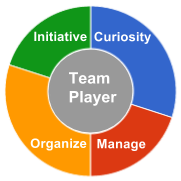
\includegraphics[scale=0.80]{img/personal.png}\\
\sectionsep

\end{minipage}
\hfill
\begin{minipage}[t]{0.66\textwidth} 

%%%%%%%%%%%%%%%%%%%%%%%%%%%%%%%%%%%%%%
%     EXPERIENCE
%%%%%%%%%%%%%%%%%%%%%%%%%%%%%%%%%%%%%%

\section{ \textcolor{gray}{\ding{58}} Experience}

\runsubsection{Coursera}
\descript{| KPCB Fellow + Software Engineering Intern }
\location{Expected June 2014 – Sep 2014 | Mountain View, CA}
\vspace{\topsep} % Hacky fix for awkward extra vertical space
\begin{tightemize}\item 52 out of 2500 applicants chosen to be a KPCB Fellow 2014.
\end{tightemize}
\sectionsep

\runsubsection{Google}
\descript{| Software Engineering Intern }
\location{May 2013 – Aug 2013 | Mountain View, CA}
\begin{tightemize}
\item Worked on the YouTube Captions team in primarily vanilla Javascript and Python to plan, design and develop the full stack implementation of a new framework to add and edit Automatic Speech Recognition captions.\item Created a backbone.js-like framework for the Captions editor.\item All code was reviewed, perfected, and pushed to production.\end{tightemize}
\sectionsep
%%%%%%%%%%%%%%%%%%%%%%%%%%%%%%%%%%%%%%
%     RESEARCH
%%%%%%%%%%%%%%%%%%%%%%%%%%%%%%%%%%%%%%

\section{ \textcolor{gray}{\ding{58}} Research}
\runsubsection{Cornell Robot Learning Lab}
\descript{| Head Undergrad Research}
\location{Jan 2014 – Present | Ithaca, NY}
Worked with \textbf{\href{http://www.cs.cornell.edu/~ashesh/}{Ashesh Jain}} and \textbf{\href{http://www.cs.cornell.edu/~asaxena/}{Prof Ashutosh Saxena}} to create \textbf{PlanIt}, a tool which  learns from large scale user preference feedback to plan robot trajectories in human environments.  Publication submitted.
\sectionsep

\runsubsection{Cornell Phonetics Lab}
\descript{| Head Undergraduate Researcher}
\location{Mar 2012 – May 2013 | Ithaca, NY}
Lead the development of \textbf{QuickTongue}, the first ever breakthrough tongue-controlled game with \textbf{\href{http://conf.ling.cornell.edu/~tilsen/}{Prof Sam Tilsen}} to aid in Linguistics research. Publication submitted.
\sectionsep

\end{minipage}
\end{document}  
\documentclass[]{article}
